% Created 2026-09-11 Fri 11:51
% Intended LaTeX compiler: pdflatex
\documentclass[11pt]{article}
\usepackage[utf8]{inputenc}
\usepackage[T1]{fontenc}
\usepackage{graphicx}
\usepackage{longtable}
\usepackage{wrapfig}
\usepackage{rotating}
\usepackage[normalem]{ulem}
\usepackage{amsmath}
\usepackage{amssymb}
\usepackage{capt-of}
\usepackage{hyperref}
\usepackage[newfloat]{minted}
\author{Dickie Smalls}
\date{\today}
\title{}
\hypersetup{
 pdfauthor={Dickie Smalls},
 pdftitle={},
 pdfkeywords={},
 pdfsubject={},
 pdfcreator={Emacs 31.0.50 (Org mode 9.7.11)}, 
 pdflang={English}}
\begin{document}

\tableofcontents

\section{Introduction}
\label{sec:org8f7b774}
\section{Boids}
\label{sec:orgd29aa5e}
Boids (short for bird-oids, or just birds pronounced with a new york accent) consists of many bird-like (hence the name) objects moving together
\begin{itemize}
\item Every boid has a position, and a velocity vector, the immediate behaviour of one boid is determined solely by its current state and by the states of nearby boids
\item In the scope of one simulation tick all boid behaviours are computed as if in parallel
\end{itemize}
\subsection{General Procedure, and Parallel Patterns Tehrein}
\label{sec:org0d749a0}
We have implemented a simpler "force field based" approach compared to the original boids paper, this simpler approach has the same parallel characteristics, it just lacks the more physics and control theory based bird simulation of the original paper, this is a shame but the bird simulation didn't introduce any aspects of interest for this exam, so it was skipped.

The procedure is as follows
\begin{itemize}
\item For all boids \texttt{x}
\begin{itemize}
\item If it's too close to the area edge or outside of the area, add a force to going back to the area center
\item For all other boids \texttt{y} (\(O(n^2)\))
\begin{itemize}
\item If \texttt{y} is too close to \texttt{x}, add a repelling force to \texttt{x} so they don't collide
\item If \texttt{y} is close enough to \texttt{x} add it as a neighbour of \texttt{x}
\end{itemize}
\item Add a force to \texttt{x} to move its position closer to the average position of its neighbours
\item Add a force to \texttt{x} to move its velocity closer to the average velocity of its neighbours
\end{itemize}
\end{itemize}

The original boids paper goes over several approaches for combining these forces (there called "potentials", as they act in a more contorl theory enviroment), we have opted for a naive weighted sum, followed by clamping of the boid's velocity.

Update computations for one all boids within a tick are indepenant of each other, as they all depend on the same state, that being the state for the previous tick, and do not modify the state they depend on.
It therefore falls under a map parallel programming pattern, and may be considered "embarassingly parallel".

\newpage
\section{Implementation}
\label{sec:org4414dc3}
\subsection{General Schema}
\label{sec:orgf4abc52}
Our implementation of the boid algorithms proceeds as follows
\begin{itemize}
\item We have two fixed size buffers of boids (number of boids stays fixed throughout simulation)
\begin{itemize}
\item One is to contain the current state of the simulation
\item One is for writing the state of the simulation in the following tick
\end{itemize}
\end{itemize}
then at every simulation tick
\begin{itemize}
\item For all boids `x` in the first buffer (hic est parallelism)
\begin{itemize}
\item Compute next state of `x`
\item Write next state of `x` in second buffer
\end{itemize}
\item Swap buffers for next iteration
\end{itemize}
\subsection{Technologies Used}
\label{sec:orgeb2abb6}
Program has been developed using C and the OpenMP library/compiler extension, due to use of OpenMP, the sequential and parallel versions of the program can use the same code base, and compilation of the code into one or the other versions may be controlled by turn OpenMP `\#pragma`s on or off by changing passed compiler flags.
\begin{quote}
\textbf{NOTE}: this produces compilation warnings for unrecognized pragmas but these warnings are of little concern
\end{quote}
Benchmark and graphical versions for the program have been developed, the graphical versions use raylib to handle the graphics
\subsection{Version Implemented}
\label{sec:org547c569}
Two versions of simulation code have been developed
\begin{itemize}
\item one where the data storing the boids, and the simulation loop following it, have data arranged in an AoS (array of structs) manner.
\item one where the data storing the boids, and the simulation loop following it, have data arranged in SoA (struct of arrays) manner.
\end{itemize}
\section{Results and Benchmarks}
\label{sec:orgacc55ca}
Benchmarks have been run using
\begin{itemize}
\item 1000 boids
\item 100 warmup iterations
\item 1000 timed iterations
\end{itemize}
Given these parameters, runtime has been measured for different numbers of openmp threads, namely 1, 2, 4, 8, and 16 threads for the parallel versions, sequential versions of the code were also benchmarked with the same amount of boids, warmup iterations, and timed iterations.

Benchmark results are as follows
\begin{center}
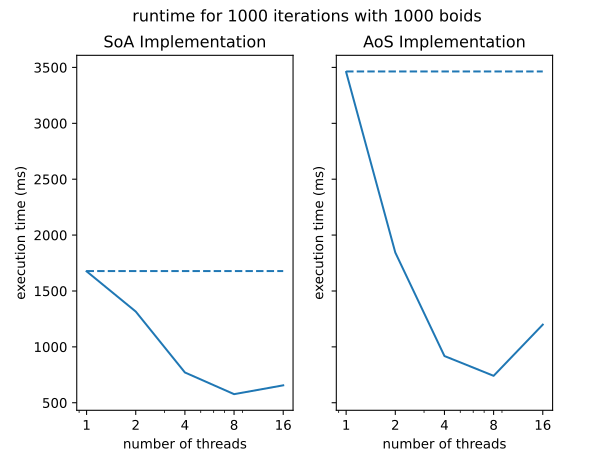
\includegraphics[width=.9\linewidth]{../presentazione/assets/images/boid-perf.png}
\end{center}
\subsection{Conclusions}
\label{sec:orgbd5dbaa}
Prefacing that the the test machine this has been run on has 8 cores, we may see that
\begin{itemize}
\item Adding threads reduces runtime as long as thread number does not exceed number of machine cores, after which increasing threads adds overhead, likely due to excessive context switching.
\item Parallel execution with only one thread matches time of sequential execution, meaning syncrhonization overhead in the 1 thread case may be considered negligeable (given our test configuration)
\item SoA version of simulation loop scores better than AoS version of the simulation loop for all tried sizes, likely due to better data locality
\end{itemize}
\end{document}
